%--------------------------------------------------------------------
% NE 155 (intro to numerical simulation of radiation transport)
% Spring 2014

% formatting
\documentclass[12pt]{article}
\usepackage[top=1in, bottom=1in, left=1in, right=1in]{geometry}

\usepackage{setspace}
\onehalfspacing

\setlength{\parindent}{0mm} \setlength{\parskip}{1em}


% packages
\usepackage{amssymb}
%% The amsthm package provides extended theorem environments
\usepackage{amsthm}
\usepackage{epsfig}
\usepackage{times}
\renewcommand{\ttdefault}{cmtt}
\usepackage{amsmath}
\usepackage{graphicx} % for graphics files

% Draw figures yourself
\usepackage{tikz} 
\usetikzlibrary{petri}

% The float package HAS to load before hyperref
\usepackage{float} % for psuedocode formatting
\usepackage{xspace}

% from Denovo methods manual
\usepackage{mathrsfs}
\usepackage[mathcal]{euscript}
\usepackage{color}
\usepackage{array}

\usepackage[pdftex]{hyperref}

\newcommand{\nth}{n\ensuremath{^{\text{th}}} }
\newcommand{\ve}[1]{\ensuremath{\mathbf{#1}}}
\newcommand{\macro}{\ensuremath{\Sigma}}
\newcommand{\vOmega}{\ensuremath{\hat{\Omega}}}
\newcommand{\Macro}{\ensuremath{\Sigma}}

\newcommand{\cc}[1]{\ensuremath{\overline{#1}}}
\newcommand{\ccm}[1]{\ensuremath{\overline{\mathbf{#1}}}}


%--------------------------------------------------------------------
%--------------------------------------------------------------------
\begin{document}
\begin{center}
{\bf NE 155, Classes 27, 28, S14 \\
2-D Finite Difference/Volume methods\\ 
April 2 \& 4, 2014}
\end{center}

\setlength{\unitlength}{1in}
\begin{picture}(6,.1) 
\put(0,0) {\line(1,0){6.25}}         
\end{picture}

Much of this can be found in Duderstadt and Hamilton Chp.\ 5 Section II.B. 

%-------------------------------------------------------------
\section{PDEs}

We'll start by considering PDEs in general, and then move on to the Diffusion Equation specifically.

A partial differential equation is an equation containing an unknown function of two or more variables and its derivatives with respect to those variables. 

If the PDE is linear in $u$ and all derivatives of $u$, then we say that the PDE is linear.
%
\begin{equation}
A\frac{\partial^2 u}{\partial x^2} + B\frac{\partial^2 u}{\partial x \partial  y} + C\frac{\partial^2 u}{\partial y^2} + D\frac{\partial u}{\partial x} + E\frac{\partial u}{\partial y} + Fu = G \nonumber
\end{equation}
%
This equation is a \textbf{2nd order} PDE in two variables. It is \textbf{linear} if $A$ through $G$ do not depend on $u$ (they may depend on $x$ and $y$).

%-------------------------------------------------------------
\vspace*{1em}

Recall that we can classify PDEs based on the geometric behavior of their solutions. \\
\underline{Note:} these classifications only apply to second order PDEs. 

\begin{itemize}
\item Elliptic if $B^2 - 4 AC < 0$. 

\item Hyperbolic if $B^2 - 4 AC > 0$

\item Parabolic if $B^2 - 4 AC = 0$
\end{itemize}

%-------------------------------------------------------------
\subsection{Elliptic Equations}

Recall that the 2-D Laplacian for the function$u(x,y)$ is
%
\begin{equation}
\nabla^2 u(x,y) = \frac{\partial^2 u}{\partial x^2} + \frac{\partial^2 u}{\partial y^2} = u_{xx} + u_{yy} \nonumber
\end{equation}
%
The Laplacian is used in many of the equations that are commonly found in physics:
%
\begin{itemize}
\item Laplace's equation
\[\nabla^2 u(x,y) = 0\]

\item Poisson's equation 
\[\nabla^2 u(x,y) = g(x,y)\]

\item Helmholtz's equation
\[\nabla^2 u(x,y) +f(x,y)u(x,y) = g(x,y)\]
\end{itemize}

% -----------------------------------------------------
\subsection{Meshing}

We will use 5 points to define our differenced Laplacian:

\begin{minipage}{0.5\textwidth}
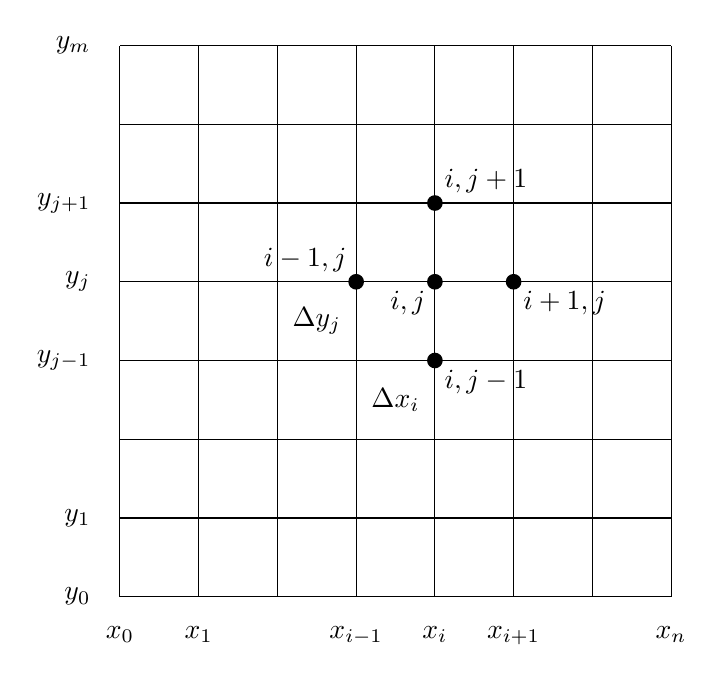
\begin{tikzpicture}
\draw (0,0)--(0,7);
\draw (1,0)--(1,7);
\draw (2,0)--(2,7);
\draw (3,0)--(3,7);
\draw (4,0)--(4,7);
\draw (5,0)--(5,7);
\draw (6,0)--(6,7);
\draw (7,0)--(7,7);
\node[below] at (0,-.25) {$x_0$};
\node[below] at (1,-.25) {$x_1$};
\node[below] at (3,-.25) {$x_{i-1}$};
\node[below] at (4,-.25) {$x_i$};
\node[below] at (5,-.25) {$x_{i+1}$};
\node[below] at (7,-.25) {$x_n$};
\node at (3.5, 2.5) {$\Delta x_i$};
% begin y
\draw (0,0)--(7,0);
\draw (0,1)--(7,1);
\draw (0,2)--(7,2);
\draw (0,3)--(7,3);
\draw (0,4)--(7,4);
\draw (0,5)--(7,5);
\draw (0,6)--(7,6);
\draw (0,7)--(7,7);
\node[left] at (-.25, 0) {$y_0$};
\node[left] at (-.25,1) {$y_1$};
\node[left] at (-.25,3) {$y_{j-1}$};
\node[left] at (-.25,4) {$y_j$};
\node[left] at (-.25,5) {$y_{j+1}$};
\node[left] at (-.25,7) {$y_m$};
  \node at (2.5,3.5) {$\Delta y_j$};
% labels
\node at (4,4) [circle,fill=black,scale=0.6] {};
\node[below left] at (4,4) {$i,j$};
\node at (5,4) [circle,fill=black,scale=0.6] {};
\node[below right] at (5,4) {$i+1,j$};
\node at (3,4) [circle,fill=black,scale=0.6] {};
\node[above left] at (3,4) {$i-1,j$};
\node at (4,5) [circle,fill=black,scale=0.6] {};
\node[above right] at (4,5) {$i,j+1$};
\node at (4,3) [circle,fill=black,scale=0.6] {};
\node[below right] at (4,3) {$i,j-1$};
\end{tikzpicture}
\end{minipage} \hfill
%
\begin{minipage}{0.5\textwidth}
  \[u(x_i,y_j) = u_{i,j} \qquad u(x_{i+1},y_j) = u_{i,j}\]
  \begin{align}
  \frac{\partial^2 u_{i,j}}{\partial x^2} = \frac{\partial}{\partial x}\bigl(\frac{\partial u_{i,j}}{\partial x}\bigr) =
\frac{u_{i-1,j} - 2u_{i,j} + u_{i+1,j}}{\Delta x_i^2} \nonumber \\
%
  \frac{\partial^2 u_{i,j}}{\partial y^2} = \frac{\partial}{\partial y}\bigl(\frac{\partial u_{i,j}}{\partial y}\bigr) =
\frac{u_{i,j-1} - 2u_{i,j} + u_{i,j+1}}{\Delta y_j^2} \nonumber
\end{align}
\end{minipage}

All together this gives
\[\nabla^2 u_{i,j} = 
\frac{\partial^2 u_{i,j}}{\partial x^2} + \frac{\partial^2 u_{i,j}}{\partial y^2} = 
\frac{u_{i-1,j} - 2u_{i,j} + u_{i+1,j}}{\Delta x_i^2} + \frac{u_{i,j-1} - 2u_{i,j} + u_{i,j+1}}{\Delta y_j^2}\]
%
If $\Delta x_i = $ constant $= \Delta y_j = h$, then
%
\[ \nabla^2 u_{i,j} = \frac{u_{i+1,j} + u_{i-1,j} + u_{i,j+1} + u_{i,j-1} - 4u_{i,j}}{h^2}\]

If we apply this to Laplace's equation and have fixed boundary conditions:
%
\begin{align}
u_{i+1,j} &+ u_{i-1,j} + u_{i,j+1} + u_{i,j-1} - 4u_{i,j} = 0 \:, i = 1, 2, \dots, n-1 \:, j = 1, 2, \dots, m-1 \nonumber \\
%
u_{0,j} &= BC_L \:, j = 1, 2, \dots, m-1 \nonumber \\
u_{i,0} &= BC_B \:, i = 1, 2, \dots, n-1 \nonumber \\
u_{n,j} &= BC_R \:, j = 1, 2, \dots, m-1 \nonumber \\
u_{i.m} &= BC_T \:, i = 1, 2, \dots, n-1 \nonumber
\end{align}
%
And make sure to check how the corners need to be defined. We could apply this directly the the 2-D diffusion equation.

%--------------------------------------------------------------------
\section{2-D Finite Volume Method, Diffusion Equation}

Remember that in 1-D we were solving this
\[-\frac{d}{dx}D(x)\frac{d \phi(x)}{dx} + \Sigma_a(x) \phi(x) = S(x)\]
%
with an equilibrium (reflecting) condition at the centerline ($x_0 = 0$) and vacuum on the right ($x_n = a$):
\begin{align}
\frac{d}{dx}\phi(x) \big|_{x=0} &= 0 \qquad \text{zero net current} \nonumber\\
\phi(\tilde{a}) &= 0 \qquad \tilde{a} = a + 2D \nonumber
\end{align}

We imposed a spatial mesh and said material discontinuities will coincide with the cell edges, $x_i$. Thus, we can assume that the cross sections and the diffusion coefficient are constant in each cell:
%
\begin{align}
D(x) &= D_i \qquad \text{for } x_{i-1} \leq x_i \nonumber \\
\Sigma_{a}(x) &= \Sigma_{a,i} \qquad \text{for } x_{i-1} \leq x_i \nonumber \\
h_i &\equiv x_i - x_{i-1} \nonumber 
\end{align}
%
The unknown fluxes and known sources are defined at the mesh or cell edges:
\begin{align}
\phi(x_i) &= \phi_i \nonumber \\
S(x_i) &= S_i \nonumber 
\end{align}
%
We then went on to define things for the finite volume method
\begin{center}
\begin{figure}[h!]
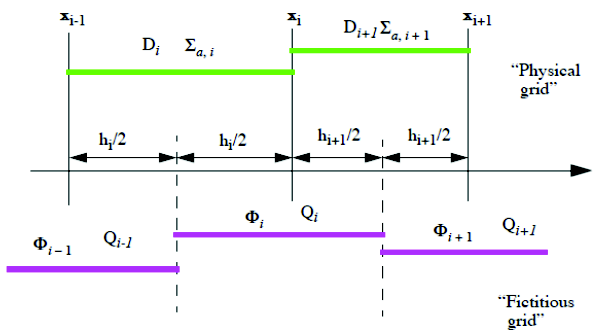
\includegraphics[height=2.5in]{FVM-DE}
\end{figure}
\end{center}

Now, we're going to extend all of this to two dimensions. We'll start with the multi-D equation:
\[-\nabla \cdot \bigl(D(\vec{r})\nabla \phi(\vec{r})\bigr) + \Sigma_a(\vec{r}) \phi(\vec{r}) = S(\vec{r})\]
%
This equation is elliptic:
\begin{itemize}
\item in general, this is the Helmholtz equation.
\item if $\Sigma_a(\vec{r})=0$ and $D(\vec{r})=$ constant, then this takes the form of the Poisson equation.
\item if $\Sigma_a(\vec{r})=0$ and $S(\vec{r})=0$, then this becomes Laplace's equation. 
\end{itemize}

In 2-D:
\[-\frac{\partial}{\partial x}D(x,y)\frac{\partial}{\partial x} \phi(x,y) + \Sigma_a(x,y) \phi(x,y) = S(x,y)\]
%
For now we're going to say we have fixed boundary conditions:
\[\phi(-a,y) = \Phi_L\:, \quad \phi(a,y) = \Phi_R\:, \quad \phi(x,-b) = \Phi_B\:, \quad \phi(x,b) = \Phi_T\:.\]
with $x \in [-a,a]$ and $y \in [-b,b]$.


% ---------------------------------------------------------
% ---------------------------------------------------------
\subsection{Finite Volume}

\begin{figure}[h!]
\begin{center}
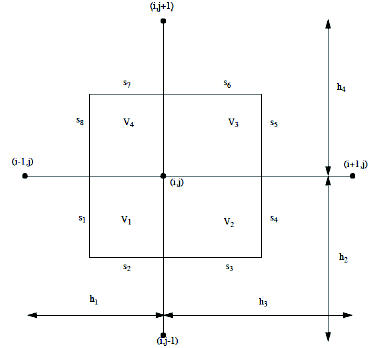
\includegraphics[height=5in]{2DfvmGrid}
\end{center}
\end{figure}

We assume the diffusion coefficient, absorption cross section, and source are constant in each cell (cell-centered), e.g., for $V_{i,j}$:
\begin{align}
D(x,y) &= D_{i,j}\;, \qquad x_{i-1} \leq x \leq x_i \:\text{ and }\: y_{j-1} \leq y \leq y_j \nonumber \\
%
\Sigma_a(x,y) &= \Sigma_{a,i,j}\;, \qquad x_{i-1} \leq x \leq x_i \:\text{ and }\: y_{j-1} \leq y \leq y_j \nonumber \\
%
S(x,y) &= S_{i,j}\;, \qquad x_{i-1} \leq x \leq x_i \:\text{ and }\: y_{j-1} \leq y \leq y_j \nonumber \\
%
\Delta x_i &\equiv \delta_i = x_{i} - x_{i-1} \nonumber \\
\Delta y_j &\equiv \epsilon_j = y_{j} - y_{j-1} \nonumber
\end{align}
And analogously for the other 3 cells.

We further assume that the fluxes are constant over the interval centered around $(x_i, y_j)$ (edge-centered):
%
\[\phi(x,y) = \phi_{i,j} \qquad \text{for } \bigl(x_i - \frac{\delta_i}{2}\bigr) \leq x \leq \bigl(x_i + \frac{\delta_{i+1}}{2}\bigr) \:\text{ and }\:\bigl(y_j - \frac{\epsilon_j}{2}\bigr) \leq x \leq \bigl(y_j + \frac{\epsilon_{j+1}}{2}\bigr) \]

Now, we integrate the 2-D equation over 4 rectangular partial-volumes (well, areas, technically): $V = V_{i,j} + V_{i+1,j} + V_{i,j+1} + V_{i+1,j+1}$.
%
\[\int_V d\vec{r}\:\bigl[-\nabla \cdot \bigl(D(\vec{r})\nabla \phi(\vec{r})\bigr) +\Sigma_a(\vec{r}) \phi(\vec{r}) = S(\vec{r}) \bigr]\]


% ---------------------------------------------------------
\subsubsection{Streaming Term}
Use Gauss Theorem to replace the first volume integral with a surface integral:
%
\begin{align}
-\int_V d\vec{r}\:\bigl[\nabla \cdot \bigl(D(\vec{r})\nabla \phi(\vec{r})\bigr)\bigr] &= -\int_S d\vec{S} \cdot\bigl(D(\vec{r})\nabla \phi(\vec{r})\bigr) \nonumber \\
%
= -\int_S d\vec{S}\: D(\vec{r})\hat{n} \cdot \nabla \phi(\vec{r}) &= -\int_S d\vec{S} \:D(\vec{r})\frac{\partial}{\partial \hat{n}}\phi(\vec{r}) \nonumber
\end{align}
%
Next, we define the partial derivative w.r.t.\ direction on each surface, using $O(h)$ forward and backward difference schemes since they're simple:

\begin{align}
\frac{\partial}{\partial \hat{n}}\phi(\vec{r}) &= \frac{\phi_{i,j-1} - \phi_{i,j}}{\epsilon_j} \qquad \text{on } S_2 \:, S_3 \nonumber \\
%
&= \frac{\phi_{i,j+1} - \phi_{i,j}}{\epsilon_{j+1}} \qquad \text{on } S_7 \:, S_6 \nonumber \\
%
&= \frac{\phi_{i-1,j} - \phi_{i,j}}{\delta_{i}} \qquad \text{on } S_1 \:, S_8 \nonumber \\
%
&= \frac{\phi_{i+1,j} - \phi_{i,j}}{\delta_{i+1}} \qquad \text{on } S_4 \:, S_5 \nonumber 
\end{align}
%
We then use the midpoint rule for the integration and integrate along each surface. Recall that the physics values are cell-centered while the flux is edge-centered. E.g., surfaces $S_2$ and $S_3$:
%
\[-\int_{S_2+S_3} d\vec{S} \:D(\vec{r})\frac{\partial}{\partial \hat{n}}\phi(\vec{r}) = \boxed{\frac{\phi_{i,j} - \phi_{i,j-1}}{\epsilon_{i}} \biggl(\frac{D_{i,j} \delta_{i} + D_{i+1,j} \delta_{i+1}}{2}\biggr)}\:,\]
%
and we do this for each set of surfaces. 


% ---------------------------------------------------------
\subsubsection{Absorption Term}
To integrate absorption, we do 4 integrals - one over each sub-volume:
%
\begin{align}
\int_{x_i-\frac{\delta_{i}}{2}}^{x_i+\frac{\delta_{i+1}}{2}} dx \int_{y_j-\frac{\epsilon_{j}}{2}}^{y_j+\frac{\epsilon_{j+1}}{2}}dy\:\Sigma_a(x,y) \phi(x,y) &= \Sigma_{a,i,j}\int\int_{V_{i,j}} dx dy \: \phi(x,y) + \nonumber \\
%
\Sigma_{a,i+1,j}\int\int_{V_{i+1,j}} dx dy \: \phi(x,y) &+ \Sigma_{a,i+1,j+1}\int\int_{V_{i+1,j+1}} dx dy \: \phi(x,y) + \nonumber \\
 \Sigma_{a,i,j+1}\int\int_{V_{i,j+1}} dx dy \: \phi(x,y) \:.\nonumber
\end{align}
%
Again applying the midpoint scheme and using our edge-centered flux definition:
%
\begin{align}
\int \int dx dy\:\Sigma_a(x,y) \phi(x,y) &= \boxed{\phi_{i,j}\bigl(\Sigma_{a,i,j} V_{i,j} + \Sigma_{a,i+1,j} V_{i+1,j} + \Sigma_{a,i+1,j+1} V_{i+1,j+1} + \Sigma_{a,i,j+1} V_{i,j+1} \bigr) } \nonumber \\
&\equiv \Sigma_{a,ij}\:, \nonumber
\end{align}
%
where
\[V_{i,j} = \frac{1}{4}\delta_i \epsilon_j \:, \quad V_{i+1,j} = \frac{1}{4}\delta_{i+1} \epsilon_{j} \:, \quad V_{i+1,j+1} = \frac{1}{4}\delta_{i+1} \epsilon_{j+1} \:, \quad V_{i,j+1} = \frac{1}{4}\delta_{i} \epsilon_{j+1} \:.\]


% ---------------------------------------------------------
\subsubsection{Source Term}
Using the same procedure for the source, we get:
\begin{align}
\int \int dx dy \: \:S(x,y) &= \boxed{ S_{i,j} V_{i,j} + S_{i+1,j} V_{i+1,j} + S_{i+1,j+1} V_{i+1,j+1} + S_{i,j+1} V_{i,j+1} }\nonumber \\
&\equiv S_{ij}\:. \nonumber
\end{align}


% ---------------------------------------------------------
\subsubsection{Discretized Equations}
Collecting all of the terms and separating them, we get a 5-point difference equation for $i=1,\dots,n-1$; $j=1,\dots,m-1$:
%
\[a_{i-1,j}^{ij}\phi_{i-1,j} + a_{i+1,j}^{ij}\phi_{i+1,j} + a_{i,j-1}^{ij}\phi_{i,j-1} + a_{i,j+1}^{ij}\phi_{i,j+1} +  a_{i,j}^{ij}\phi_{i,j} = S_{i,j} \]
%
the lower index is the cell to which you are coupling, and the upper index is which cell you are in - this becomes important when we're ordering our matrix.
%
\begin{align}
a_{i-1,j}^{ij} &= -\frac{D_{i,j} \epsilon_{j} + D_{i,j+1} \epsilon_{j+1}}{2 \delta_{i}}  \nonumber \\
(a_L^{ij} & \quad \text{capturing influence of \textbf{left} flux on center cell}) \nonumber \\
%
a_{i+1,j}^{ij} &= -\frac{D_{i+1,j} \epsilon_{j} + D_{i+1,j+1} \epsilon_{j+1}}{2 \delta_{i+1}}  \nonumber \\
(a_R^{ij} & \quad \text{capturing influence of \textbf{right} flux on center cell}) \nonumber \\
%
a_{i,j-1}^{ij} &= -\frac{D_{i,j} \delta_{i} + D_{i+1,j} \delta_{i+1}}{2 \epsilon_{j}}  \nonumber \\
(a_B^{ij} & \quad \text{capturing influence of \textbf{lower} flux on center cell}) \nonumber \\
%
a_{i,j+1}^{ij} &= -\frac{D_{i,j+1} \delta_{i} + D_{i+1,j+1} \delta_{i+1}}{2 \epsilon_{j+1}}  \nonumber \\
(a_T^{ij} & \quad \text{capturing influence of \textbf{upper} flux on center cell}) \nonumber \\
%
a_{i,j}^{ij} &= \Sigma_{a,ij} - \bigl(a_{i-1,j}^{ij} + a_{i+1,j}^{ij} + a_{i,j-1}^{ij} + a_{i,j+1}^{ij} \bigr)
 \:.\nonumber \\
 (a_C^{ij}) & \nonumber
\end{align}

In this formulation we now have $(n+1) \times (m+1)$ unknowns. 

%-------------------------------------------------------
\subsection{Matrix Form}
To write the system in a way that looks like $\ve{A}\vec{x} = \vec{b}$, we need to choose an ordering strategy for how we want to store the points. Let's look at a 3$\times$3 example:

\begin{minipage}{0.5\textwidth}
%-------------- indices ------------------
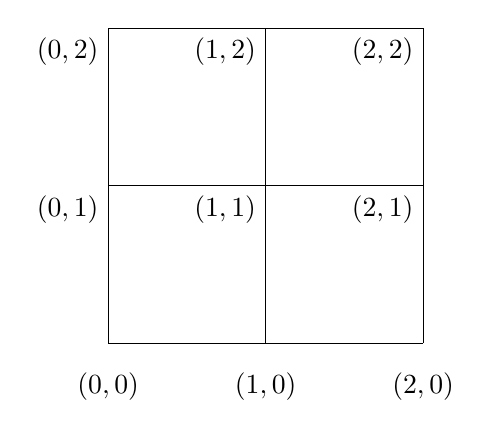
\begin{tikzpicture}
\draw[step=2cm] (0,0) grid (4,4);
\foreach \y in {1, 2}
    \foreach \x in  {0, 1, 2}
        \node[below left] at (2*\x cm,2*\y cm) {$(\x,\y)$};
\node[below] at (0,-.25) {$(0,0)$};
\node[below] at (2,-.25) {$(1,0)$};
\node[below] at (4,-.25) {$(2,0)$};
\end{tikzpicture}
\end{minipage} \hfill
%-------------- numbered nodes ------------------
\begin{minipage}{0.5\textwidth}
\begin{tikzpicture}
\draw[step=2cm] (0,0) grid (4,4);
\node[below] at (0,-.25) {$0$};
\node[below] at (2,-.25) {$1$};
\node[below] at (4,-.25) {$2$};
\node[below left] at (-.25,2) {$3$};
\node[below left] at (2,2) {$4$};
\node[below left] at (4,2) {$5$};
\node[below left] at (-.25,4) {$6$};
\node[below left] at (2,4) {$7$};
\node[below left] at (4,4) {$8$};
\end{tikzpicture}
\end{minipage}

Our solution vector length in this example is 9 (3 $\times$ 3). Our matrix size is therefore going to be 9 $\times$ 9. We can think of this as a 3 $\times$ 3 matrix of 3 $\times$ 3 matrices:
\begin{equation}
\underbrace{\begin{pmatrix}
\begin{pmatrix}
a_{0,0}^{00} & a_{1,0}^{00} & 0 \\
a_{0,0}^{10} & a_{1,0}^{10} & a_{2,0}^{10} \\
0            & a_{1,0}^{20} & a_{2,0}^{20}
\end{pmatrix} 
&
\begin{pmatrix}
a_{0,1}^{00} & 0 & 0 \\
0 & a_{1,1}^{10} & 0 \\
0 & 0 & a_{2,1}^{20}
\end{pmatrix}
&
\begin{pmatrix}
 & & \\
 & 0 & \\
 & & 
\end{pmatrix} \\
%--------------------
\begin{pmatrix}
a_{0,0}^{01} & 0 & 0 \\
0 & a_{1,0}^{11} & 0 \\
0 & 0 & a_{2,0}^{21}
\end{pmatrix}
&
\begin{pmatrix}
a_{0,1}^{01} & a_{1,1}^{01} & 0 \\
a_{0,1}^{11} & a_{1,1}^{11} & a_{2,1}^{11} \\
0            & a_{1,1}^{21} & a_{2,1}^{21}
\end{pmatrix}
&
\begin{pmatrix}
a_{0,2}^{01} & 0 & 0 \\
0 & a_{1,2}^{11} & 0 \\
0 & 0 & a_{2,2}^{21}
\end{pmatrix} \\
%--------------------
\begin{pmatrix}
 & & \\
 & 0 & \\
 & & 
\end{pmatrix} &
\begin{pmatrix}
a_{0,1}^{02} & 0 & 0 \\
0 & a_{1,1}^{12} & 0 \\
0 & 0 & a_{2,1}^{22}
\end{pmatrix}
&
\begin{pmatrix}
a_{0,2}^{02} & a_{1,2}^{02} & 0 \\
a_{0,2}^{12} & a_{1,2}^{12} & a_{2,2}^{12} \\
0            & a_{1,2}^{22} & a_{2,2}^{22}
\end{pmatrix} \\
\end{pmatrix}}_{\ve{A}}
%--------------------
%
\underbrace{\begin{pmatrix} \phi_{0,0} \\ \phi_{1,0} \\ \phi_{2,0} \\ \\ \phi_{0,1} \\ \phi_{1,1} \\ \phi_{2,1} \\ \\ \phi_{0,2}\\ \phi_{1,2} \\  \phi_{2,2} \end{pmatrix}}_{\vec{\phi}} =
%
\underbrace{\begin{pmatrix} S_{0,0} \\ S_{1,0} \\ S_{2,0} \\ \\ S_{0,1} \\ S_{1,1} \\ S_{2,1} \\ \\ S_{0,2} \\ S_{1,2} \\  S_{2,2} \end{pmatrix}}_{\vec{S}} \nonumber
\end{equation}

%
%
Another way to think of $\ve{A}$ is
\begin{equation}
\begin{pmatrix}
\begin{pmatrix}
a_{C}^{00} & a_{R}^{00} & 0 \\
a_{L}^{10} & a_{C}^{10} & a_{R}^{10} \\
0            & a_{L}^{20} & a_{C}^{20}
\end{pmatrix} 
&
\begin{pmatrix}
a_{T}^{00} & 0 & 0 \\
0 & a_{T}^{10} & 0 \\
0 & 0 & a_{T}^{20}
\end{pmatrix}
&
\begin{pmatrix}
 & & \\
 & 0 & \\
 & & 
\end{pmatrix} \\
%--------------------
\begin{pmatrix}
a_{B}^{01} & 0 & 0 \\
0 & a_{B}^{11} & 0 \\
0 & 0 & a_{B}^{21}
\end{pmatrix}
&
\begin{pmatrix}
a_{C}^{01} & a_{R}^{01} & 0 \\
a_{L}^{11} & a_{C}^{11} & a_{R}^{11} \\
0            & a_{L}^{21} & a_{C}^{21}
\end{pmatrix}
&
\begin{pmatrix}
a_{T}^{01} & 0 & 0 \\
0 & a_{T}^{11} & 0 \\
0 & 0 & a_{T}^{21}
\end{pmatrix} \\
%--------------------
\begin{pmatrix}
 & & \\
 & 0 & \\
 & & 
\end{pmatrix} &
\begin{pmatrix}
a_{B}^{02} & 0 & 0 \\
0 & a_{B}^{12} & 0 \\
0 & 0 & a_{B}^{22}
\end{pmatrix}
&
\begin{pmatrix}
a_{C}^{02} & a_{R}^{02} & 0 \\
a_{L}^{12} & a_{C}^{12} & a_{R}^{12} \\
0            & a_{L}^{22} & a_{C}^{22}
\end{pmatrix} \\
\end{pmatrix} \nonumber
\end{equation}

This gives us a 5-banded matrix, which is not so difficult to represent with built in functions. We could still solve this directly with Gaussian elimination or LU decomposition, but the size of the system increases pretty rapidly with mesh size.

Therefore using an iterative method like Jacobi, GS, or SOR is probably a better plan. 


%-------------------------------------------------------
\subsection{Boundary Conditions}

This all works fine for central points, but what about the boundaries? When we're at the edges, we get 4 entries rather than 5 because the edge values are know. For corners we have only 3 entries. 

Let's see how this impacts our equations. Recall:
%
\[\phi(-a,y) = \Phi_L\:, \quad \phi(a,y) = \Phi_R\:, \quad \phi(x,-b) = \Phi_B\:, \quad \phi(x,b) = \Phi_T\:.\]
%
Let's choose what to do at the corners, and then define the rest of the boundaries:
\[\phi_{0,0} = \Phi_B\:, \quad \phi_{0,m} = \Phi_R\:, \quad \phi_{0,m} = \Phi_L\:, \quad \phi_{n,m} = \Phi_T\:.\]
%
\begin{align}
\phi_{0,j} &= \Phi_L \qquad j=1,\dots,m-1 \nonumber \\
\phi_{n,j} &= \Phi_R \qquad j=1,\dots,m-1 \nonumber \\
\phi_{i,0} &= \Phi_B \qquad i=1,\dots,n-1 \nonumber \\
\phi_{i,m} &= \Phi_T \qquad i=1,\dots,n-1 \nonumber \\
\end{align}

Let's look at how this would impact the left ($i=0$) boundary. The $i=0$ equations are simply the boundary condition:
\begin{itemize}
\item Change the $a_{C}^{0,j}$ entries to $1$s, 
\item the $a_{x}^{0,j}$, where $x$ is $R, T, B$ to $0$, and 
\item the $S_{0,j}$ entries to $\Phi_L$.
\end{itemize} 

For the $i=1$ equations:
\[\underbrace{a_{2,j}^{1j}}_{R}\phi_{2,j} + \underbrace{a_{1,j-1}^{1j}}_{B}\phi_{1,j-1} + \underbrace{a_{1,j+1}^{1j}}_{T}\phi_{1,j+1} + \underbrace{a_{1,j}^{1j}}_{C}\phi_{1,j} = S_{1,j} - \underbrace{a_{0,j}^{1j}}_{L}\phi_L \]

And analogously for the rest of the edges.

%--------------------------------------------------------------------
%--------------------------------------------------------------------
%\bibliographystyle{plain}
%\bibliography{LinearSolns} 

\end{document}